\chapter{数据处理和分析}
\section{PIN阵列数据与准弹性散射角分布}



% 根据硅阵列数据得到的准弹性散射角分布
在实验中，PIN探测器的能量分辨约0.4~MeV，无法直接区分出弹性散射反应道与准弹性散射反应道对应的峰。因此，能量谱主峰中至少包含了$^{152}\mathrm{Sm}(^{18}\mathrm{O},^{18}\mathrm{O})^{152}\mathrm{Sm}_{0^+}$、$^{152}\mathrm{Sm}(^{18}\mathrm{O},^{18}\mathrm{O})^{152}\mathrm{Sm}_{2^+}$、$^{152}\mathrm{Sm}(^{18}\mathrm{O},^{18}\mathrm{O})^{152}\mathrm{Sm}_{4^+}$反应道的计数。另外，实验中为了让靶始终面向Q3D磁谱仪的入口，需要不断旋转靶角，导致总有一些角度的硅探测器与靶框形成较大的角度，并使得谱中显示出大幅度的低能拖尾。
因此，对谱中主峰进行了拖尾高斯拟合，以期望尽可能在各轮数据间一致地得到峰计数，拖尾高斯函数表达式为：

\begin{multline}
f(x; A, t, u, c) = \frac{A}{2t} \, \exp\!\left( \frac{x-u}{t} + \frac{c^2}{2t^2} \right) \cdot \\
 \operatorname{erfc}\!\left( \frac{1}{\sqrt{2}} \left( \frac{x-u}{c} + \frac{c}{t} \right) \right)
\end{multline}
其中$\mu$、c与标准高斯函数的均值、标准差相对应，函数经过设计使得A恰好为函数的积分，t则对应函数拖尾的程度。指数拖尾部分主要描述探测器死层、靶框遮挡及电荷收集不完全带来的低能展宽。
图\ref{pin}为$E_\mathrm{lab} = 72$~MeV下由位于45°的硅探测器得到的能量谱。

\begin{figure}[h]
\centering
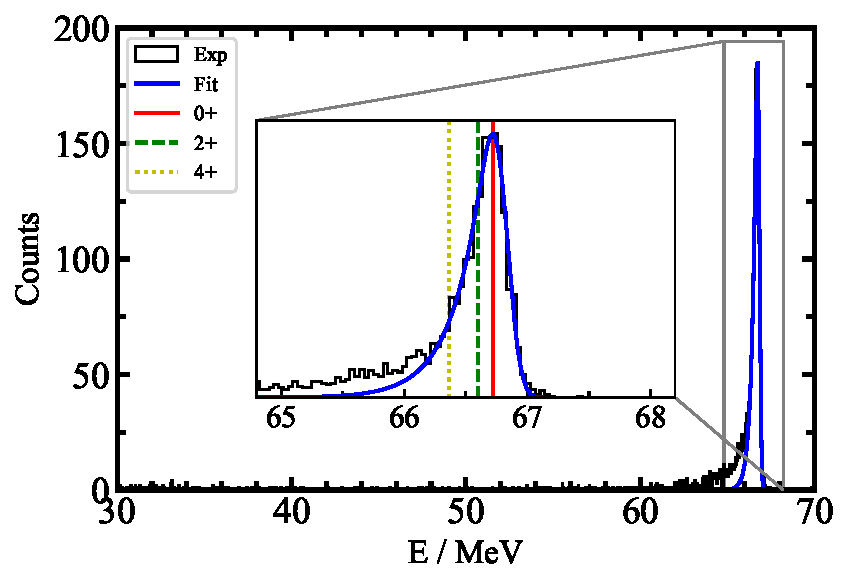
\includegraphics[width=0.8\linewidth]{images/pin_with_inset.pdf}
\caption{典型的pin探测器能量谱}
\small 阶梯线段为实验数据，曲线表示拖尾高斯的拟合结果，详情图中从高能到低能的三条竖线分别表示$0^+$、$2^+$、$4^+$三个反应道出射粒子总能量对应的峰位。PIN探测器的能量分辨无法直接区分出三个反应道对应的峰，对应计数用于准弹性散射角分布。
\label{pin}
\end{figure}
最终结果在图\ref{result}中使用矩形点表示，误差仅考虑统计误差。尽管这种数据处理方法可以应对探测器与靶框角度过大的问题，但也可能将额外的反应道计数加入到准弹性散射的总计数中，这为基于硅阵列数据得到的角分布带来了一些误差。这些误差在垒下的能点较为明显，体现为相对截面的值存在一些涨落。
\section{焦面探测器数据与弹性散射角分布}


\begin{figure*}
\centering
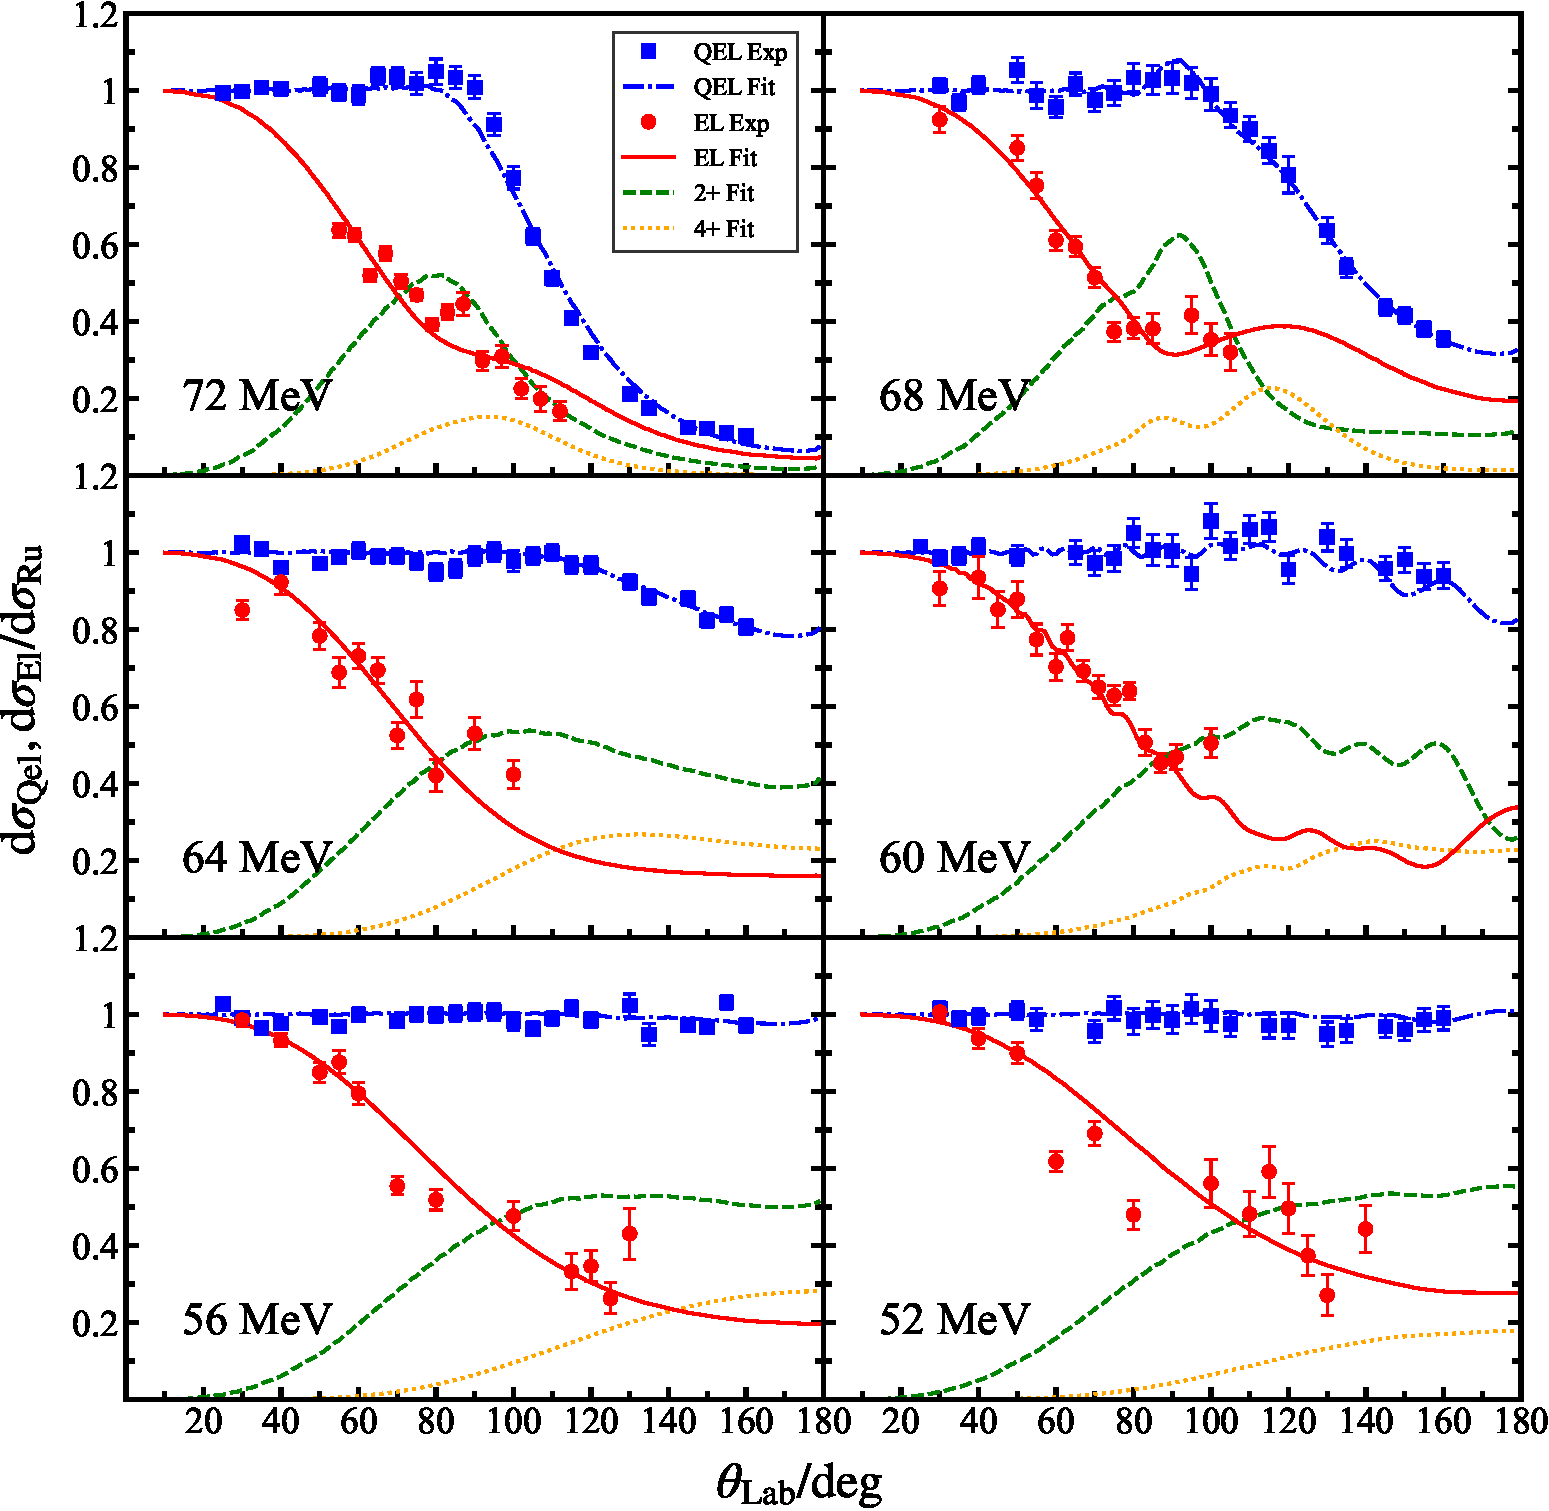
\includegraphics[width=1.1\linewidth]{images/result.pdf}
\caption{各个能量下实验和预测的准弹性散射以及弹性散射截面}
\small 图中矩形为实验准弹性散射角分布，圆形为实验弹性散射角分布，曲线中点划线表示模型预测的准弹性散射角分布，实线表示预测的弹性散射角分布，虚线表示预测的$4^+$反应道截面的角分布，点线表示预测的$2^+$反应道截面的角分布
\label{result}
\end{figure*}
% }
使用Q3D磁谱仪搭配焦面探测器的探测体系对弹核质量、探测器摆放位置等实验细节因素非常敏感。本次实验缺乏有效的调试工具以及充分的束流时间，导致未能获得最理想的分辨。尽管如此，相较于PIN阵列，Q3D磁谱仪系统还是具有更高的动量分辨能力，因此可进一步提取纯弹性散射信息。图\ref{focal}为$E_\mathrm{lab} = 60$~MeV下，Q3D角度为66°时，焦面探测器得到的位置谱。由图可见，最终的分辨无法将$^{152}\mathrm{Sm}(^{18}\mathrm{O},^{18}\mathrm{O})$ $^{152}\mathrm{Sm}_{0^+}$与$^{152}\mathrm{Sm}(^{18}\mathrm{O},^{18}\mathrm{O})^{152}\mathrm{Sm}_{2^+}$两个反应道对应的峰直接分开，因此需要通过多高斯拟合来得到各个反应道的计数。

拟合的函数可以表示为：
\begin{multline}
f(x) = G(x,A_{\mathrm{0^+}},\mu_{\mathrm{0^+}},\sigma_{\mathrm{0^+}}) + G(x,A_{2^+},\mu_{2^+},\sigma_{2^+}) \\
+ G(x,A_{4^+},\mu_{4^+},\sigma_{4^+})
\end{multline}
其中
$$
G(x,A,\mu,\sigma) = A e^{-\frac{(x-\mu)^2}{2\sigma^2}}
$$
为标准高斯函数，而$x$则为焦面探测器的位置，$f(x)$为一个合适的分bin下$x$位置对应的计数。

这里同时对三个反应道进行高斯拟合，一共需要得到9个参数。由于$^{152}\mathrm{Sm}$三个态的能量展宽都很小，因此假定三个峰的展宽相同，也就是
$$
\sigma_{\mathrm{0^+}} = \sigma_{2^+} = \sigma_{4^+}
$$
另外，因为已知三个反应道的能量差，在动量刻度后就可以确定三个峰之间的位置差，于是最终只需要拟合5个参数：$\mu_{\mathrm{0^+}},\sigma_{\mathrm{0^+}},A_{\mathrm{0^+}},A_{2^+},A_{4^+}$。拟合得到的各个高斯函数用曲线绘制在图\ref{focal}中。

\begin{figure}[h]
\centering
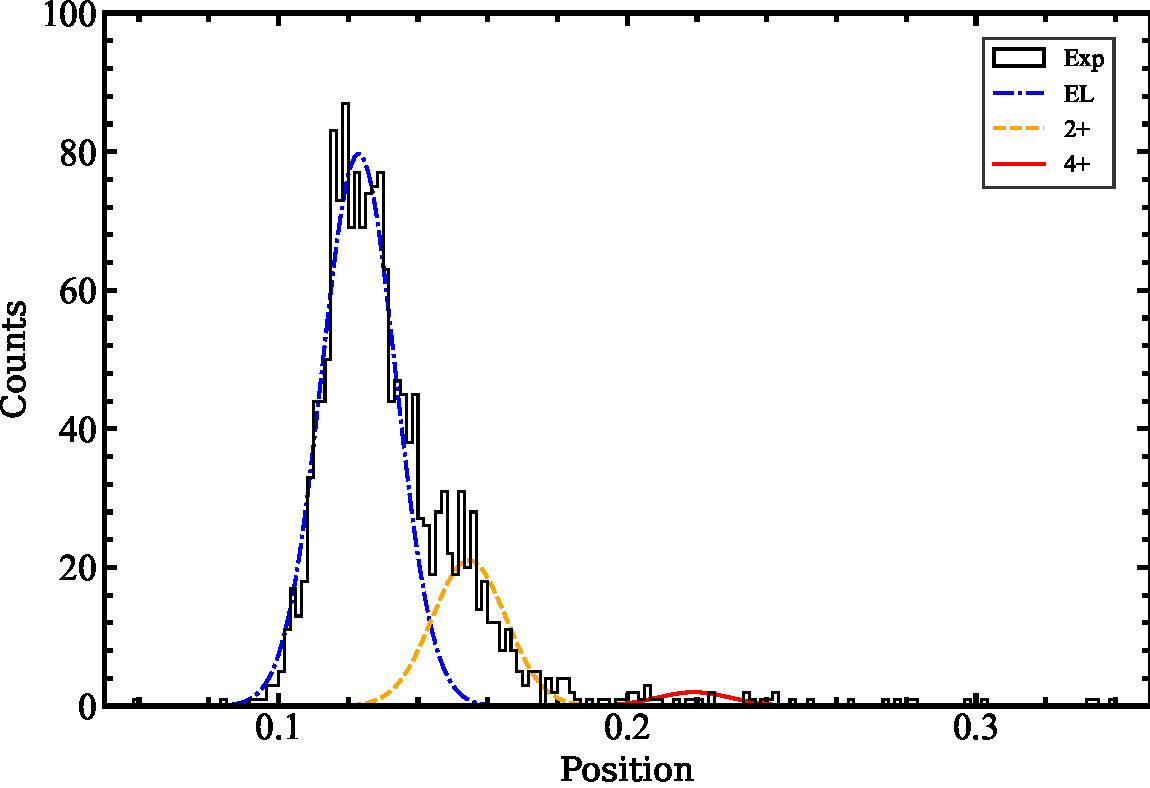
\includegraphics[width=0.7\linewidth]{images/focal.pdf}
\caption{焦面探测器位置谱}
\small 负方向为高能端，正方向为低能端，阶梯线段为实验数据，从高能到低能端的三条曲线表示多高斯拟合$0^+$、$2^+$、$4^+$三个反应道的结果。
\label{focal}
\end{figure}
最终得到的弹性散射角分布在图\ref{result}中使用圆形点表示，误差仅考虑统计误差。从$^{152}\mathrm{Sm}(^{18}\mathrm{O},^{18}\mathrm{O}_{\mathrm{0^+}})$反应的弹性散射角分布数据中，可以观察到很强的库仑虹抑制。这一现象与大形变体系$^{16}\mathrm{O}+^{152}\mathrm{Sm}$\cite{kim1979nuclear,talon1981coulomb}、$^{18}\mathrm{O}+^{184}\mathrm{W}$\cite{thorn1977effect}中的观测结果一致。
% 这里可以加几个例子


\section{光学势参数的拟合}




使用光学模型对准弹性散射和弹性散射的实验数据进行同时拟合，可以得到每一个能量下的光学势参数。使用的光学模型的相互作用势$U(r)$可以表示为：
\begin{equation}
U(r)= V_C(r) - V_0f(r,R_V,a_V) - iW_0f(r,R_W,a_W)
\label{opt}
\end{equation}
其中，$V_C$为弹核与靶核之间的库仑势，一般可以用一个特定半径的电荷均匀分布的库仑场来表示：
\begin{equation}
V_C(r) = 
\begin{cases} 
\dfrac{(3R_C^2 - r^2) Z_P Z_T e^2}{2R_C^3}, & r < R_C \\[1em]
\dfrac{Z_P Z_T e^2}{r}, & r \geq R_C 
\end{cases}
\end{equation}
其中半径$R_C=r_C(A_T^{1/3}+A_P^{1/3})$，$r_C$为约化库仑半径，$A_T,A_P,Z_T,Z_P$分别为靶核和弹核的质量数和电荷数。

而光学势中的$V_0f(r,R_V,a_V)$和$iW_0f(r,R_W,a_W)$即为实部和虚部势，都通常分成深度和形状因子两个部分。$V_0$和$W_0$分别为实部和虚部的势深度，$f$则为实部和虚部的形状因子，一般可以采用Woods-Saxon势的形式：
\begin{equation}
f(r, R_i, a_i) = \left[ 1 + \exp\left(\frac{r - R_i}{a_i}\right) \right]^{-1}
\end{equation}

\begin{equation}
R_i = r_i(A_P^{1/3} + A_T^{1/3}) \quad i = V, W
\end{equation}
于是，这个光学势一共有6个待定参数，分别为实部的$V_0$、$r_V$、$a_V$和虚部的$W_0$、$r_W$和$a_W$。

在实际拟合中，使用的约化库仑半径$r_C=1.25$~fm\cite{kim1979nuclear}，以及在两个不同来源中一致的形状因子参数：$r_V=2.02~fm$，$r_W=2.06~fm$，$a_V=0.5~fm$，$a_W=0.55~fm$\cite{kim1979nuclear,talon1981coulomb}。每个能点只需要对两个势深度参数进行拟合。

ECIS95 是 J. Raynal 开发的核反应计算程序，可用于光学模型与耦合道计算，在重离子散射数据分析中被广泛采用\cite{raynal1994ecis}。该程序能够在给定核势参数与耦合方案的条件下，计算弹性散射及非弹激发角分布，并通过实验数据比较提取光学势参数。
本工作中使用ECIS95程序对实验准弹性散射和弹性散射角分布数据进行双参数拟合，得到了每个能点的实部$V_0$和虚部的势深度$W_0$。其中，在ECIS的输入文件中使用了$\beta_2 = 0.308$，$\beta_4 = 0.127$作为四极形变参数和八极形变参数，考虑了对称转动耦合。详细的ECIS95输入文件如下：
\begin{lstlisting}
 O18+Sm152  EL=72MEV  OPT SERCH (inc. tar. 2^+, 4^+)
TFFFFFFFFFTTFFFTFFFFFFFFFFFFTFTTTFFFFFFFFFFTFFFFFF 
FFFFFFFFFFFFFFFFFFFFTTFFTFFFFFFFFFFFFFFFTFFFFFFFFF 
    3  400   40              4    4 
0.1       50. 
0.     1  72.       0.        18.       152.      496. 
2.     1  0.121782
4.     1  0.366479
    2    4        0. 
0.308     0.127
10.62     1.37      0.50 
5.74      1.40      0.55 
 
1.25 

      10.0       1.0     179.0
    4    2    3  200      20.0       1.0
F1 14    1    1
      55.0    0.6373    0.0180       0.1       0.1
      59.0    0.6244    0.0165       0.1       0.1
      63.0    0.5192    0.0158       0.1       0.1
      67.0    0.5767    0.0169       0.1       0.1
      71.0    0.5045    0.0176       0.1       0.1
      75.0    0.4691    0.0143       0.1       0.1
      79.0    0.3925    0.0154       0.1       0.1
      83.0    0.4235    0.0194       0.1       0.1
      87.0    0.4455    0.0310       0.1       0.1
      92.0    0.2982    0.0248       0.1       0.1
      97.0    0.3095    0.0290       0.1       0.1
     102.0    0.2251    0.0257       0.1       0.1
     107.0    0.1989    0.0332       0.1       0.1
     112.0    0.1668    0.0247       0.1       0.1
F1  0    3    0
F1  0    2    0
F1 25    1    0
      25.0  27847.60    195.36       0.1       0.1
      30.0  13670.79    200.05       0.1       0.1
      35.0   7579.17    119.93       0.1       0.1
      40.0   4514.31     75.43       0.1       0.1
      50.0   1947.54     45.22       0.1       0.1
      55.0   1342.97     27.71       0.1       0.1
      60.0    970.98     23.95       0.1       0.1
      65.0    764.74     16.23       0.1       0.1
      70.0    586.47     13.30       0.1       0.1
      75.0    454.12     13.12       0.1       0.1
      80.0    376.20     11.68       0.1       0.1
      85.0    303.34      8.47       0.1       0.1
      90.0    246.28      7.24       0.1       0.1
      95.0    188.15      5.95       0.1       0.1
     100.0    136.69      5.07       0.1       0.1
     105.0     95.24      3.07       0.1       0.1
     110.0     69.09      2.45       0.1       0.1
     115.0     48.94      2.04       0.1       0.1
     120.0     34.44      1.61       0.1       0.1
     130.0     18.96      1.30       0.1       0.1
     135.0     14.52      0.89       0.1       0.1
     145.0      9.08      0.60       0.1       0.1
     150.0      8.42      0.57       0.1       0.1
     155.0      7.28      0.54       0.1       0.1
     160.0      6.57	  0.51       0.1       0.1
      0.01      0.01     
    1    4   
FIN
\end{lstlisting}


% \begin{figure}
% \centering
% \includegraphics[width=1\linewidth]{images/72.pdf}
% \caption{拟合结果与参考文献的对比}
% \small 图中方形为实验准弹性散射角分布，圆形为实验弹性散射角分布，实线表示本工作模型预测的结果，虚线表示Talon等的结果，点划线表示Kim的结果，点线表示Zhao等的结果。
% \label{72}
% \end{figure}
\section{光学势的能量相依性与色散关系}

将上一节中ECIS95拟合得到的参数重新代入表达式~\eqref{opt}中，可以得到模型预测的各个反应道的反应截面，在图\ref{result}中用曲线表示。
从图中可以看到，模型较好再现了实验角分布的整体趋势。，但是对弹性散射实验数据的拟合在后角区域仍存在明显偏差，这主要受限于弹性散射实验数据本身的误差和涨落。但是如果仅使用准弹性散射数据对光学模型参数进行拟合，失去弹性散射数据约束后的模型结果不确定性会大幅增加，特别是在垒下能点无法得到有意义的实部虚部势深度。这是因为当体系能量低于库仑势垒，相互作用过程由库仑力主导，核力的影响有限。从实验角分布可以看出，随着入射能量降低，偏离卢瑟福散射的特征角逐渐向背角移动。当体系能量低于库仑势垒后，角分布整体接近卢瑟福散射。
同时，由核库仑干涉产生的振荡结构逐渐减弱，说明核相互作用贡献显著下降，由库仑散射与核散射相干叠加引起的明暗条纹和库仑虹也变得微弱直至不可见。因此，垒下的准弹性散射数据对核势（尤其是实部）的敏感度极低，几乎不包含可以约束光学势深度的有效信息。这使得模型的可靠拟合高度依赖于弹性散射数据的约束。目前拟合结果与实验数据的整体趋势较为一致，当然在精度方面还有一些提升空间。

从$^{152}\mathrm{Sm}(^{18}\mathrm{O},^{18}\mathrm{O})^{152}\mathrm{Sm}_{2^+}$、$^{152}\mathrm{Sm}(^{18}\mathrm{O},^{18}\mathrm{O})^{152}\mathrm{Sm}_{4^+}$两个反应道角分布的拟合结果来看，模型认为在库仑激发的相对截面总是在前角随着角度增大而快速上升，这与库仑虹抑制、弹性散射相对截面的快速下降相对应，表示入射道通量就是从弹性散射流失到了库仑激发的反应道上。而随着能量降低，背角的库仑激发相对截面在逐渐上升，表示能量越低，在背角库仑激发占比就越大。这可能反映了核力的影响随着能量降低逐渐减小，库仑力逐渐占主导的结果。
% 由图\ref{72}对于72~MeV能点，拟合得到的光学势参数所给出的弹散、非弹激发曲线的趋势与$^{16}\mathrm{O}+^{152}\mathrm{Sm}$\cite{talon1981coulomb,kim1979nuclear}、$^{12}\mathrm{C}+^{152}\mathrm{Sm}$\cite{zhao1994comparison}体系中的情况基本一致————随着角度增加，弹性散射的通道被快速吸收，2+态对应的反应道截面在70-80°达到最大，而4+态则是在80-95°达到最大。这显示出以$^{152}\mathrm{Sm}$为靶核这样的大形变体系的截面变化的共同趋势。


根据拟合结果，给出了$^{18}\mathrm{O}+^{152}\mathrm{Sm}$体系在六个能点下光学势的能量相依性，如图\ref{final}所示，详细数据见表\ref{excel}。误差由卡方最小化得到的协方差矩阵的对角元计算得出。
\begin{table}[htbp]
\centering
\begin{tabular}{ccccc}
\toprule
Energy (MeV) & V (MeV) & W (MeV) & $\chi^2_{\text{Qel}}$/pt & $\chi^2_{\text{El}}$/pt \\

\midrule   

72 & 7.14 \pm 0.46 & 2.12 \pm 1.22 & 3.08 & 8.70 \\
68 & 11.09 \pm 3.55 & 0.86 \pm 1.84 & 0.63 & 2.34 \\
64 & 6.94 \pm 1.27 & 1.17 \pm 0.80 & 1.09 & 7.32 \\
60 & 25.50 \pm 4.01 & 0.66 \pm 1.03 & 1.27 & 3.23 \\
56 & 1.51 \pm 4.90 & 3.47 \pm 3.63 & 1.54 & 4.78 \\
52 & 2.47 \pm 8.32 & 7.25 \pm 4.94 & 0.59 & 7.34 \\
\bottomrule
\end{tabular}
\caption{ECIS95程序拟合得到的光学势参数及其拟合优度}
\label{excel}
\end{table}


图中实验得到的实部势深度在库仑势垒($\approx$60~MeV)附近有一个明显的凸起，这与典型的阈异常现象相似。由于能点有限并且间隔较大，还无法对实部行为给出更详细的描述。但是虚部势深度随着能量降低却反常地有抬升的趋势，这与$^{6}\mathrm{Li}+^{208}\mathrm{Pb}$体系的光学势十分相似\cite{keeley1994optical}。为了通过虚部得到实部的预测曲线，首先要对虚部进行分段线性拟合。普通的阈异常体系可以使用一个在反应阈值开始，虚部从0开始上升到一个平台的线性模型，表达式如下：
\begin{equation}
W(E) = 
\begin{cases}
0, & E \le E_a \\[1ex]
W_{0s} \, \dfrac{E - E_a}{E_b - E_a}, & E_a < E < E_b \\[1ex]
W_{0s}, & E \ge E_b
\end{cases}
\end{equation}
而实验得到的虚部势随着能量降低而抬升，这无法指示出一个反应阈值，也无法应用这样简单的线性模型。因此，此处使用一个虚部由初值下降到平台的线性模型进行拟合，表达式如下：
\begin{equation}
W(E) = 
\begin{cases}
W_{0s}, & E \le E_a \\[1ex]
W_{0s} - (W_{0s} - W_{1s}) \, \dfrac{E - E_a}{E_b - E_a}, & E_a < E < E_b \\[1ex]
W_{1s}, & E \ge E_b
\end{cases}
\end{equation}
当然，该模型仅作为一种经验性的参数化方式，用于定性检验色散关系的预期行为。
得到虚部的模型后，再通过式~\eqref{kk}计算得到了根据色散关系预测的实部理论曲线。理论曲线预测实部势深度将会在56~MeV附近达到极小值，并在60~MeV附近有一个拐点；但是实验的实部势深度是在60~MeV附近达到了极大值，拐点的位置则可能在60-64~MeV之间，实验的结果显著偏离了色散关系的预测。基于目前的数据所给出的结论是，该体系的光学势并不满足色散关系，表现出反常阈异常的特征。

值得强调的是，对于垒下的两个能点52、56~MeV，拟合得到的光学势参数误差很大。这是因为当前光学势的拟合中仅对两个势深度参数进行拟合，数据的误差会直接导致参数值的偏离。此外，尽管研究中使用的光学势形状因子参数可以一定程度地重现实验数据，但是这并不代表目前使用的就是最佳的参数，考虑到从弹性散射与准弹性散射实验数据抽取光学势参数存在Igo模糊的问题\cite{lin2015}，这可能也会加大结果的不确定性。
因此，只有基于更丰富、更精确的实验数据，并在拟合过程中更全面地考虑各参数之间的相互影响，才能得到该体系光学势行为的更有力的结论。
\begin{figure}
\centering
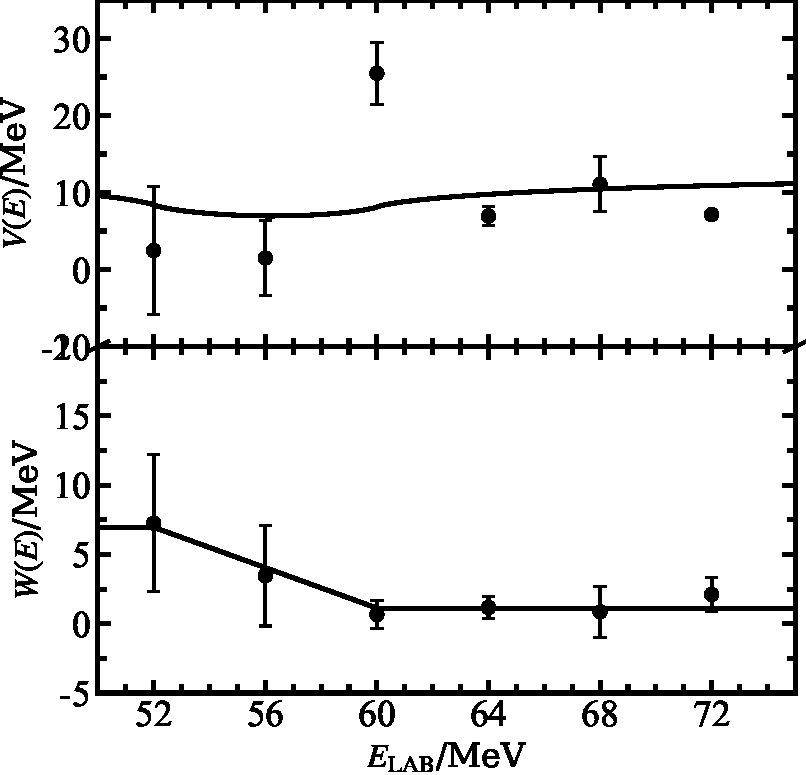
\includegraphics[width=0.7\linewidth]{images/final.pdf}
\caption{光学势的能量相依性}
\small 图中上半部分表示实部势深度，下半部分表示虚部势深度。原点表示实验值。虚部的拟合结果用线段表示，由虚部及色散关系得到的实部预测值用曲线表示。
\label{final}
\end{figure}

本章对实验获取的PIN阵列与Q3D焦面探测器数据进行了系统处理，分别提取了准弹性散射角分布与弹性散射角分布。基于耦合道光学模型，对六个能点的实验数据进行了联合拟合，获得了体系实部与虚部光学势参数的能量依赖关系。

结果表明，
$^{18}\mathrm{O}$ + $^{152}\mathrm{Sm}$体系在库仑势垒附近表现出异常的势参数变化：实部势深度出现增强，而虚部势深度未呈现常规下降趋势。进一步与色散关系比较发现，实验结果与理论预期存在明显偏离，提示该体系可能存在反常阈异常行为。